\documentclass[10pt]{beamer}

\usetheme[progressbar=frametitle]{m}

\usepackage{booktabs}
\usepackage[scale=2]{ccicons}

\usepackage{pgfplots}
\usepgfplotslibrary{dateplot}


\title{Metagenomic reconstruction of bacterial CRISPR loci constrain population histories}
\subtitle{Banfield et al.}
\date{\today}
\author{Kathryn Iverson}
\institute{Schloss Lab \\ \LaTeX}
%\titlegraphic{\hfill
\includegraphics[height=1.5cm]{logo}}

\begin{document}

\maketitle

\begin{frame}
  \frametitle{Table of Contents}
  \setbeamertemplate{section in toc}[sections numbered]
  \tableofcontents[hideallsubsections]
\end{frame}

%%%%%%%%%%%%%%%%%%%%%%%%%%%%%%%%%%%%%%%%%%%%%%%%%%%%%%%%%%%%%%%%%%%%%%%%%%%%
\begin{frame}[fragile]
	\frametitle{Overview}

Metagenomic approach to look at \emph{Leptospirillum} CRISPR loci and phage
	\begin{itemize}
        \item "detect and recover genome sequences from uncultivated phage and link phage to their hosts"
        \begin{itemize}
        	\item reconstruct phage genome from extracted spacer sequences
            \item determine who goes with whom
        \end{itemize}
        \item time series data to look at population history
    \end{itemize}

\end{frame}
%%%%%%%%%%%%%%%%%%%%%%%%%%%%%%%%%%%%%%%%%%%%%%%%%%%%%%%%%%%%%%%%%%%%%%%%%%%%
\section{CRISPR-Cas}

\begin{frame}[fragile]
  \frametitle{CRISPR-Cas}
  
  Bacterial and archaeal immune system against plasmids and phages
  \begin{figure}
  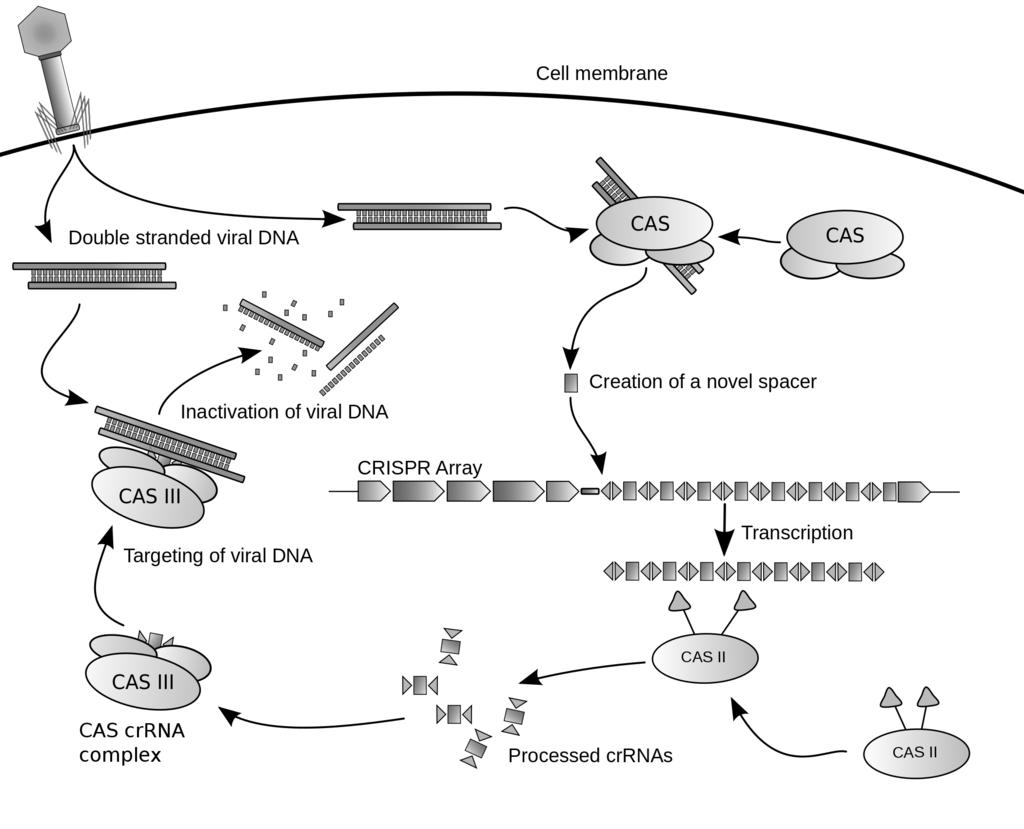
\includegraphics[width=\textwidth,height=0.6\textheight,keepaspectratio]{1024px-Crispr.png}
  \caption{Diagram of the possible mechanism for CRISPR}
  \end{figure}
  \footnote{James Atmos CC BY-SA 3.0 or GFDL, via Wikimedia Commons}

\end{frame}

%%%%%%%%%%%%%%%%%%%%%%%%%%%%%%%%%%%%%%%%%%%%%%%%%%%%%%%%%%%%%%%%%%%%%%%%%%%%
\begin{frame}[fragile]
	\frametitle{CRISPR locus}

  \begin{figure}
  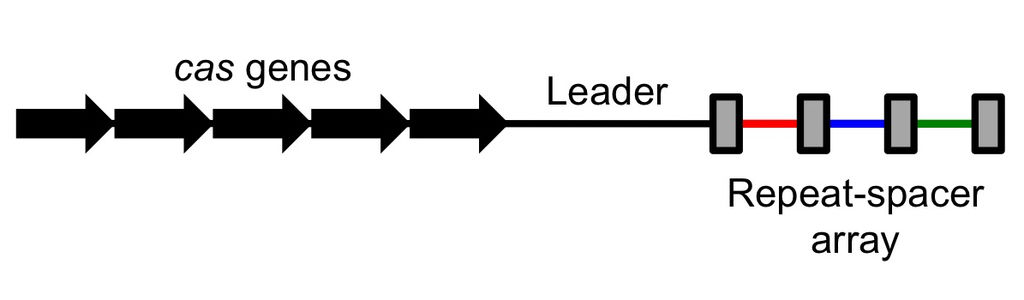
\includegraphics[width=\textwidth,height=0.6\textheight,keepaspectratio]{1024px-SimpleCRISPR.jpg}
  \caption{Simplified diagram of a CRISPR locus}
  \end{figure}
  \footnote{AnnaJune CC BY-SA 3.0 or GFDL, via Wikimedia Commons}

\end{frame}

%%%%%%%%%%%%%%%%%%%%%%%%%%%%%%%%%%%%%%%%%%%%%%%%%%%%%%%%%%%%%%%%%%%%%%%%%%%%

\section{Methods and Results}

\begin{frame}[fragile]
	\frametitle{Sampling and genomic data}
    
	\begin{itemize}
		\item 9 biofilm communities from the Richmond Mine
        \item Sanger sequencing
        \item 5way and UBA samples had \emph{Leptospirillum} group II CRISPR locus amplified with CRISPR primers and sequenced with 454
	\end{itemize}

\end{frame}

%%%%%%%%%%%%%%%%%%%%%%%%%%%%%%%%%%%%%%%%%%%%%%%%%%%%%%%%%%%%%%%%%%%%%%%%%%%%

\begin{frame}[fragile]
	\frametitle{Spacer richness and diversity}
    \begin{columns}
    \column{0.5\textwidth}
    	\begin{figure}
    		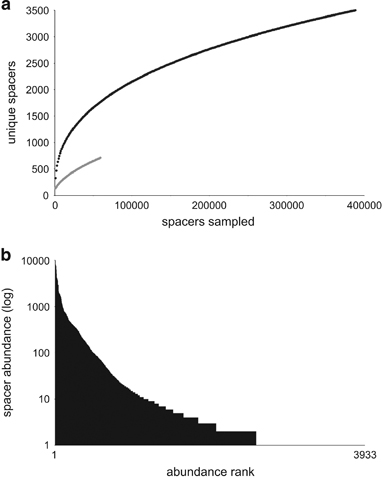
\includegraphics[width=\textwidth,height=0.6\textheight,keepaspectratio]{ismej_fig1.jpg}
    		\caption{Paper Figure 1}
    	\end{figure}
    \column{0.5\textwidth}
		\begin{itemize}
			\item Rarefaction curves don't approach saturation
            \item Due to high error rates, spacer were clustered into groups based on length and identity
            	\begin{itemize}
                	\item 3933 unique group II groups
                    \item 296 unique group III groups
                \end{itemize}
            \item most unique groups only occur a few times across all datasets
		\end{itemize}
	\end{columns}
\end{frame}
%%%%%%%%%%%%%%%%%%%%%%%%%%%%%%%%%%%%%%%%%%%%%%%%%%%%%%%%%%%%%%%%%%%%%%%%%%%%

\begin{frame}[fragile]
	\frametitle{Locus reconstruction}
    \begin{figure}
    		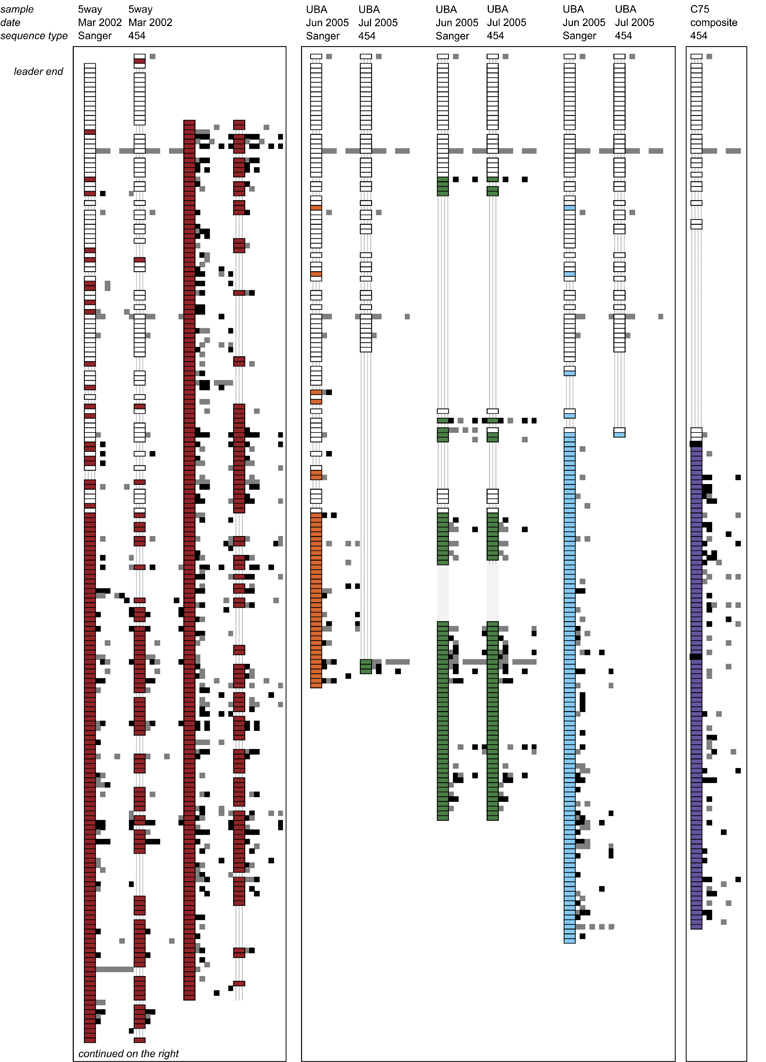
\includegraphics[width=\textwidth,height=0.9\textheight,keepaspectratio]{ismej_fig2.jpg}
    		%\caption{Paper Figure 2}
    \end{figure}

\end{frame}
%%%%%%%%%%%%%%%%%%%%%%%%%%%%%%%%%%%%%%%%%%%%%%%%%%%%%%%%%%%%%%%%%%%%%%%%%%%%

\begin{frame}[fragile]
	\frametitle{PAM sequences}
    
	\begin{itemize}
		\item PAM sequence for each \emph{Leptospirillum} group was found by comparing proto-spacer flanking sequences using WebLogo
        \item Conserved tri-nucleotide flanking sequence AAG for group II and di-nucleotide sequence AA for group III
	\end{itemize}
     \begin{figure}
    		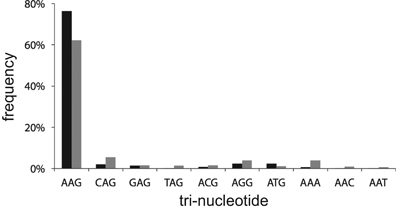
\includegraphics[width=\textwidth,height=0.6\textheight,keepaspectratio]{ismej_fig3.jpg}
    		%\caption{Paper Figure 2}
    \end{figure}

\end{frame}
%%%%%%%%%%%%%%%%%%%%%%%%%%%%%%%%%%%%%%%%%%%%%%%%%%%%%%%%%%%%%%%%%%%%%%%%%%%%

\begin{frame}[fragile]
	\frametitle{Spacer matches to genome}
    \begin{itemize}
    	\item Host self targeting
    	\item Most often 5way spacers match genes from UAB groups and vice versa
    \end{itemize}
    \begin{figure}
    		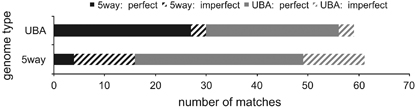
\includegraphics[width=\textwidth,height=0.6\textheight,keepaspectratio]{ismej2_fig4.jpg}
    		%\caption{Paper Figure 2}
    \end{figure}

\end{frame}
%%%%%%%%%%%%%%%%%%%%%%%%%%%%%%%%%%%%%%%%%%%%%%%%%%%%%%%%%%%%%%%%%%%%%%%%%%%%
\begin{frame}[fragile]
	\frametitle{Spacer matches to phage and mobile elements}
    Reads that don't map to CRISPR or host genome are likely from phage or mobile elements
    \begin{figure}
    		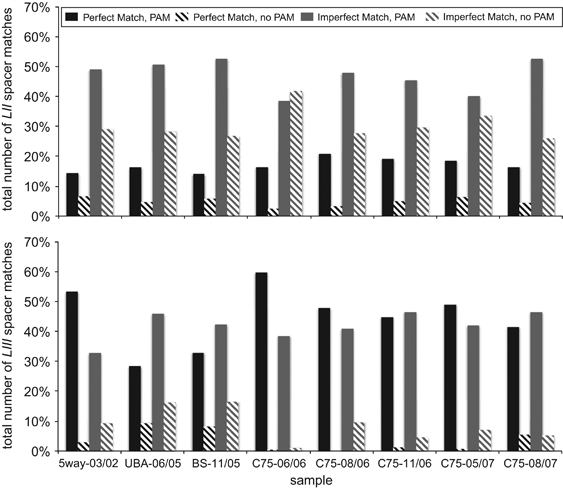
\includegraphics[width=\textwidth,height=0.6\textheight,keepaspectratio]{ismej_fig5.jpg}
    		%\caption{Paper Figure 2}
    \end{figure}
    

\end{frame}
%%%%%%%%%%%%%%%%%%%%%%%%%%%%%%%%%%%%%%%%%%%%%%%%%%%%%%%%%%%%%%%%%%%%%%%%%%%%
\begin{frame}[fragile]
	\frametitle{Spacer matches to phage and mobile elements}
    \begin{figure}
    		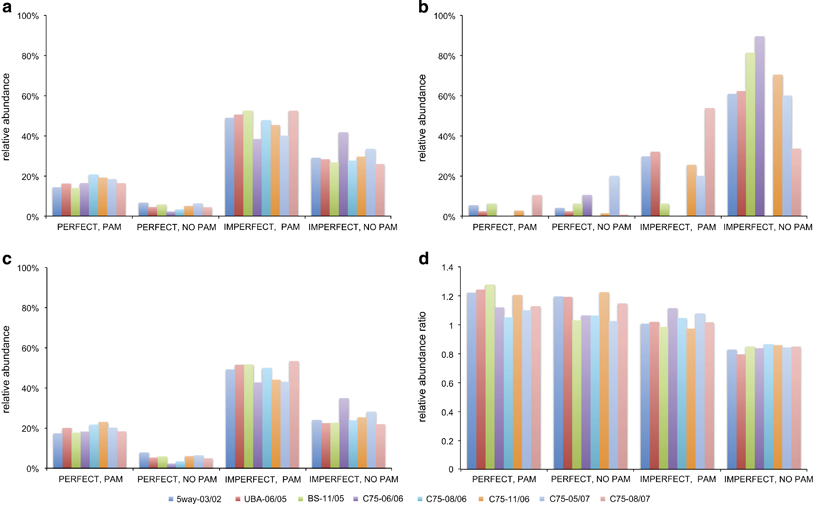
\includegraphics[width=\textwidth,height=1\textheight,keepaspectratio]{ismej_fig6.jpg}
    		%\caption{Paper Figure 2}
    \end{figure}

\end{frame}
%%%%%%%%%%%%%%%%%%%%%%%%%%%%%%%%%%%%%%%%%%%%%%%%%%%%%%%%%%%%%%%%%%%%%%%%%%%%
\begin{frame}[fragile]
	\frametitle{Spacer matches to phage and mobile elements}
    Spacers with mutations (and a perfect PAM) are 9.2 times more common than PAMs with mutations (associated with a perfect spacer)

\end{frame}
%%%%%%%%%%%%%%%%%%%%%%%%%%%%%%%%%%%%%%%%%%%%%%%%%%%%%%%%%%%%%%%%%%%%%%%%%%%%

\begin{frame}[fragile]
	\frametitle{History of targeting of the known \emph{Leptospirillum} phage AMDV1}
    
	\begin{itemize}
    	\item AMDV1 is a \emph{Leptospirillum} group II phage
		\item 9 spacers that perfectly match longest AMDV1 contig
        \item Spacer matches occur throughout all time points
        \item Blocks of spacers from June 2005 that don't contain matches, possible fluctuation in phage exposure
	\end{itemize}

\end{frame}
%%%%%%%%%%%%%%%%%%%%%%%%%%%%%%%%%%%%%%%%%%%%%%%%%%%%%%%%%%%%%%%%%%%%%%%%%%%%

\section{Discussion}

\begin{frame}[fragile]
	\frametitle{}
    
	\begin{itemize}
		\item Few self-targeting spacers, mostly to mobile elements in the genome
        \item Targets may not exist in the same genome!
        \item The trailer end \emph{Leptospirillum} group II spacers were largely conserved over the 5-year study period
        \item Most spacer diversity occurs at the leader end. Rarefaction curves show lack of saturation. Cells can contain different CRISPR loci.
	\end{itemize}

\end{frame}
%%%%%%%%%%%%%%%%%%%%%%%%%%%%%%%%%%%%%%%%%%%%%%%%%%%%%%%%%%%%%%%%%%%%%%%%%%%%

\begin{frame}[fragile]
	\frametitle{}
    CRISPR loci can provide population history 
    \begin{itemize}
		\item older and new spacers target essentially the same phage population, a result that points to the persistence of \emph{Leptospirillum} in an environment with the same phage population over the time period represented by the locus (>5 years)
        \item missing AMDV1 spacers mid locus may suggest period of fluctuation in phage exposure
        \item Spacer regions mutate before PAM at frequencies expected with random mutation
	\end{itemize}
 

\end{frame}
%%%%%%%%%%%%%%%%%%%%%%%%%%%%%%%%%%%%%%%%%%%%%%%%%%%%%%%%%%%%%%%%%%%%%%%%%%%%

\plain{Questions?}

\end{document}


